\documentclass[11pt]{article}
\usepackage[margin=1in]{geometry}
\usepackage{graphicx}
\usepackage{booktabs}
\usepackage{amsmath}
\usepackage{siunitx}
\graphicspath{{figures/}}

\title{A host-side check for an STM32N657 CNN:\\
what matches the PC, and what does not}
\author{Alexander Bashirov}
\date{20 October 2026}

\begin{document}
\maketitle

\section{Question}
The CNN used here is a small MNIST network: two \(3\times 3\) convolutions, two max-pools, and two linear layers. The same checkpoint can be run in PyTorch on the PC and on a NUCLEO-N657X0-Q. This note records one fresh on-board measurement and the host-side tools added so that a later export can be checked before it is flashed.

The score is the mean, over images, of the squared Euclidean distance between two length-10 logit vectors. Label accuracy is a different number: the fraction of images whose largest logit equals the written digit. Cosine similarity is a third number: the mean, over images, of the cosine between the two logit vectors. A large squared gap can sit next to a cosine near 1 and next to an unchanged winning class.

\section{What was run}
The board was reachable on the ST-LINK (\texttt{/dev/ttyACM0}). The firmware loaded into RAM is the CNN with FP16 weights and FP32 activations (Helium, weight-only). It is not the Cube.AI graph. The run used the project's usual subset: MNIST test images, \texttt{numpy} generator seed 0, 200 images, indices sorted, pixels divided by 255.

On the PC, the same checkpoint was evaluated twice. Once with the stored FP32 weights. Once after \texttt{stm32nn.round\_fp16}, which casts every parameter to IEEE FP16, nearest, and stores it back in FP32. \texttt{stm32nn.compare} then scored the board logits and the Cube.AI FP32 logits, already saved from the earlier serial run of the same 200 images, against the PC FP32 logits.

\section{Results}
\label{sec:results}

\begin{center}
\begin{tabular}{lrrr}
\toprule
Run & Logit MSE vs PC FP32 & Cosine & Argmax differs \\
\midrule
PC, weights rounded to FP16 & \(2.422\times 10^{-5}\) & \(1.000\) & 0/200 \\
STM32, Helium, same rounding & \(2.422\times 10^{-5}\) & \(1.000\) & 0/200 \\
STM32, Cube.AI FP32 graph & \(5.445\) & \(0.998\) & 0/200 \\
\bottomrule
\end{tabular}
\end{center}

Label accuracy is 0.995 on all three runs and on the untouched FP32 network: 199 of 200 digits. The Helium program and the PC rounding differ only in the last digits of the logit MSE (\(2.422037\times 10^{-5}\) against \(2.421720\times 10^{-5}\)). The file written by the eval script reports \(2.422138\times 10^{-5}\). Figure~\ref{fig:hist} shows that this gap is small on every image.

\begin{figure}[ht]
  \centering
  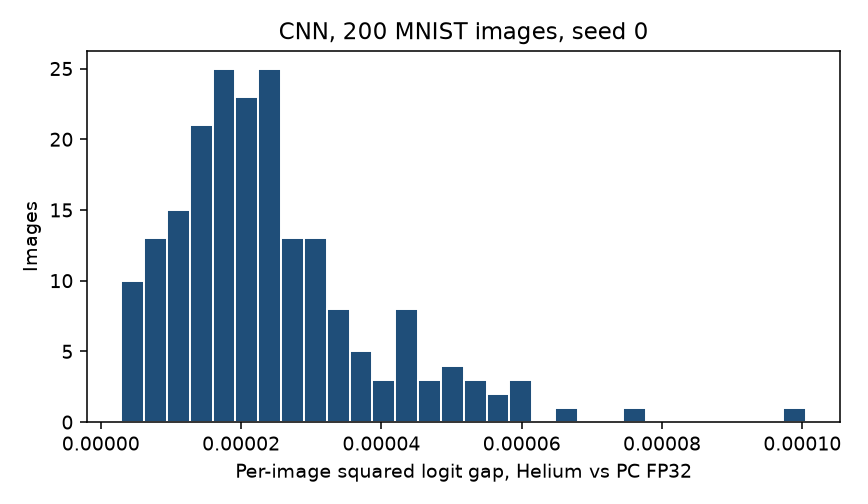
\includegraphics[width=0.78\textwidth]{helium_gap_hist.png}
  \caption{Squared logit gap of the Helium CNN against PC FP32, one bar per image.}
  \label{fig:hist}
\end{figure}

The Cube.AI FP32 graph is a different program. Its mean squared gap is about \(2\times 10^{5}\) times larger. Figure~\ref{fig:cube} is the histogram of the base-10 logarithm of that per-image gap, because the raw values span more than one decade. The cosine stays at 0.998 and the winning class does not change. The squared gap and the class decision are not substitutes.

\begin{figure}[ht]
  \centering
  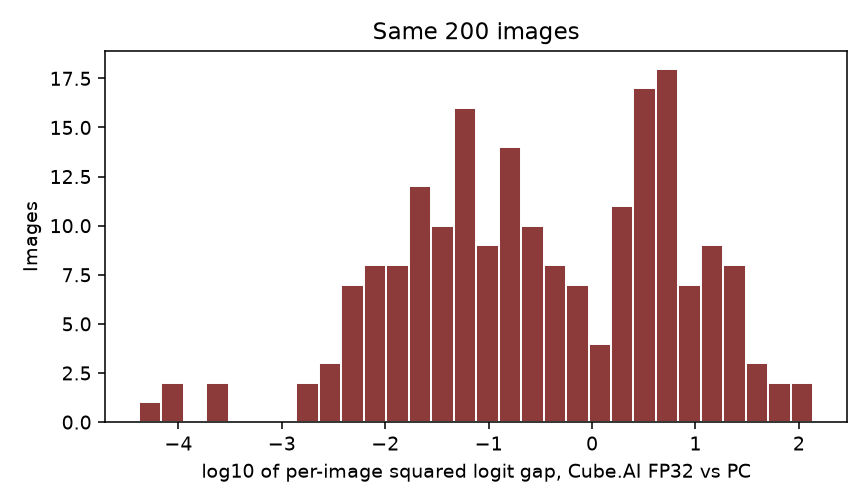
\includegraphics[width=0.78\textwidth]{cubeai_gap_hist.png}
  \caption{Cube.AI FP32 CNN against the same PC FP32 logits. The axis is logarithmic.}
  \label{fig:cube}
\end{figure}

\begin{figure}[ht]
  \centering
  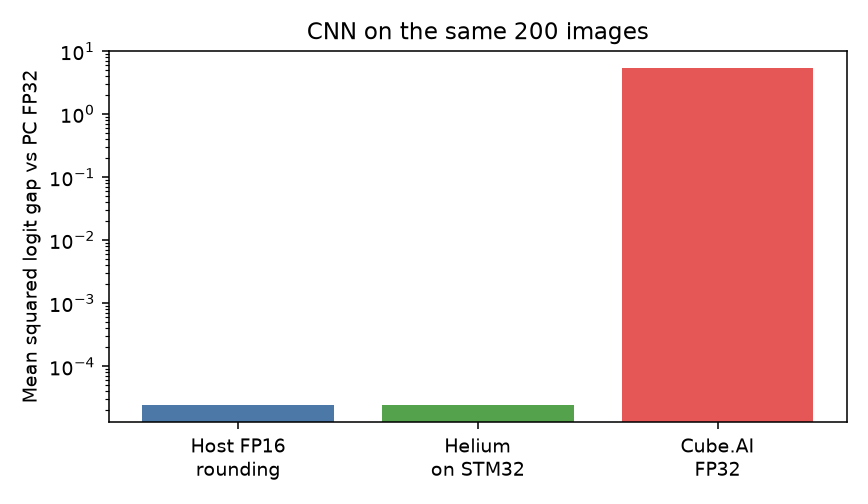
\includegraphics[width=0.72\textwidth]{mse_bars.png}
  \caption{The three gaps on one logarithmic axis. The left two bars are the FP16 rounding. The right bar is the Cube.AI FP32 graph.}
  \label{fig:bars}
\end{figure}

The run was repeated on 20 October 2026 with the board attached. The logit gaps above are unchanged. The Helium kernel time, from the firmware cycle counter and excluding the serial transfer, has mean 510.4\,ms on that run (Figure~\ref{fig:lat}).

\begin{figure}[ht]
  \centering
  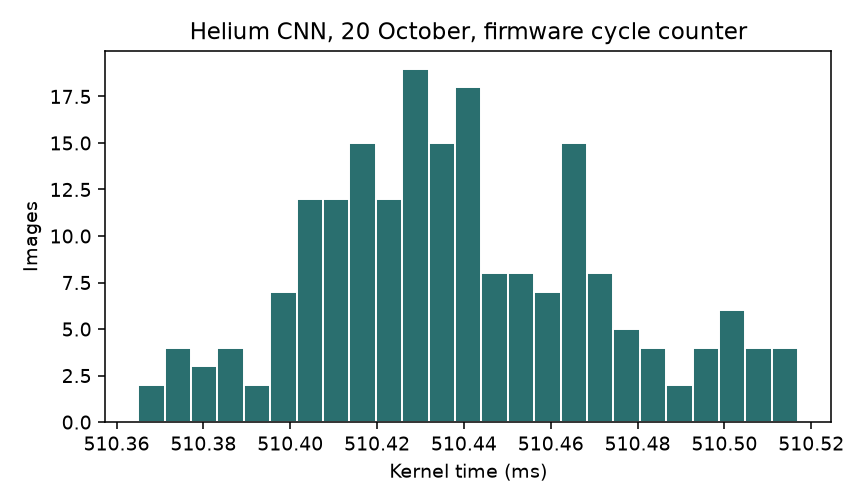
\includegraphics[width=0.72\textwidth]{latency_hist.png}
  \caption{Per-image kernel time of the Helium CNN.}
  \label{fig:lat}
\end{figure}

\section{The host extension}
\texttt{stm32nn} is a C++ PyTorch module built with CMake. It does not run on the microcontroller and it does not alter the Cube.AI graph. The operations used or added for this check are:

\begin{itemize}
  \item \texttt{round\_fp16}: IEEE FP16 nearest, stored back in FP32. This is the rounding in the left bar of Figure~\ref{fig:bars}.
  \item \texttt{to\_nhwc}, \texttt{to\_nchw}: the generated CNN buffers are channel-last. PyTorch is channel-first.
  \item \texttt{quantize\_per\_channel}: symmetric int8 along one axis.
        The scale is \(\max|w|/127\), and the codes lie in \([-127,127]\).
        The returned tensor is FP32.
        On the first convolution the mean squared change of the weights is \(5.05\times 10^{-7}\).
        That is a weight rounding, not a board measurement.
  \item \texttt{max\_pool2d}, plus the existing \texttt{conv2d} and \texttt{linear}: the generated schedule keeps convolution, ReLU, pool, and linear as separate steps.
  \item \texttt{compare}: logit MSE, argmax disagreement, and mean cosine. Section~\ref{sec:results} uses this function.
  \item \texttt{check\_export} reports a float16 parameter, a prime channel count above 64,
        a sample that is not a float image divided by 255, and an ONNX file that stores FP16.
        On this CNN and a zero \(28\times 28\) sample the list is empty.
        A 257-channel weight and a sample equal to 255 produce both warnings.
\end{itemize}

The \texttt{conv2d} and \texttt{linear} loops are a fixed FP32 accumulation written for the extension.
They are not the loop inside the Cortex-M55 network runtime library.
The generated CNN calls the float convolution inside that library.
The body of that function is not shipped as C.
Copying a guessed loop into the extension would not make the PC reproduce the Cube.AI number 5.445.

\section{What this does not claim}
The Helium result is a match between the PC rounding and the board for this one CNN, this 200-image subset, and this firmware. The Cube.AI FP32 number is from the saved serial run of the same subset, not from a new flash tonight. Closing that gap requires the generated C model to be validated on the PC with ST Edge AI, which is not installed here, or a change of the graph that is then flashed and measured again.

\end{document}
